Consider the following graph. \\
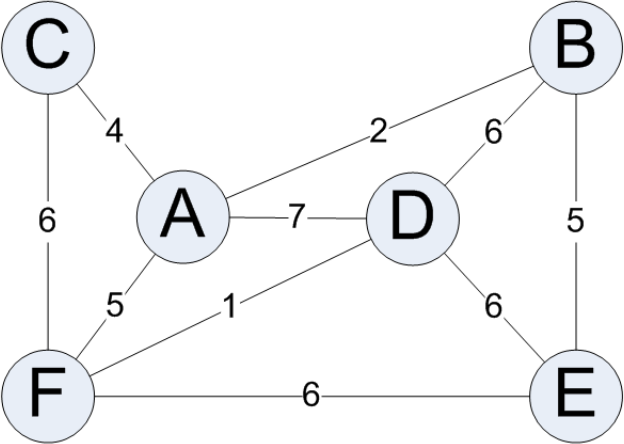
\includegraphics[height=150px]{other/graph.png}
\begin{enumerate}
	\item
	Perform Dijkstra's algorithm to find the shortest path between C and E. \\
	\def\arraystretch{1.65}
	\begin{tabu}{| c | c | c | c | c | c | c |}
		\hline
		Finalized & A & B & C & D & E & F\\
		\hline
		-- & ($\infty$, None) & ($\infty$, None) & \textbf{(0, None)} & ($\infty$, None) & ($\infty$, None) & ($\infty$, None) \\
		\answerrow{C & \textbf{(4, C)} & ($\infty$, None) & (0, None) & ($\infty$, None) & ($\infty$, None) & \textbf{(6, C)}} \\
		\answerrow{A & (4, C) & \textbf{(6, A)} & (0, None) & \textbf{(11, A)} & ($\infty$, None) & (6, C)} \\
		\answerrow{F & (4, C) & (6, A) & (0, None) & \textbf{(7, F)} & \textbf{(12, F)} & (6, C)} \\
		\answerrow{B & (4, C) & (6, A) & (0, None) & (7, F) & \textbf{(11, B)} & (6, C)} \\
		\answerrow{D & (4, C) & (6, A) & (0, None) & (7, F) & (11, B) & (6, C)} \\
		\answerrow{E & (4, C) & (6, A) & (0, None) & (7, F) & (11, B) & (6, C)} \\
		\hline
	\end{tabu} \\

	\begin{answer}
		The shortest path is CABE with a total cost of 11.
		To reconstruct this solution, we start with the destination node, then move on to its recorded optimal predecessor.
		We repeat the process until we reach the starting node.
		(Note that this isn't the only possible table.)
	\end{answer}

	\item
	In general, when using Dijkstra's algorithm to find the shortest path between nodes,
	do you need to use every row of the table? Why or why not?

	\begin{answer}
		No. The algorithm is finished as soon as the destination node has been finalized;
		Dijkstra's is a greedy algorithm so it will never change decisions once they are made.
	\end{answer}
\end{enumerate}
